
\section{Iterative Methods for Neutron Transport}
Solving the transport equation involves several nested iterative solvers. To discuss these iterative methods it is useful to think of the transport equation in operator form
\begin{equation}
    \bf{L}\psi = \bf{S}\psi + \bf{Q} \:,
\end{equation}
where $\bf{L}$ is the matrix formed by discretizing the left-hand side, $[\hat{\Omega} \cdot \nabla + \Sigma(\vec{r}, E)]\psi(\vec{r}, \hat{\Omega}, E)$, using finite elements or any other discretization method and $\bf{S}\psi$ and $\bf{Q}$ are matrices representing the source terms. 

\subsubsection{Linear Solver}
The inner-most layer of iteration is the linear solve in which the transport equation is treated as a system of linear equations and solve for a vector, $\psi$, which represents the flux at several points in space. In order to solve the equation, it must take the form ${\bf A} x = b$ where $b$ is a constant vector. In our case, $b = {\bf S} \psi + {\bf Q}$, which is dependent on $\psi$ in the scattering source and makes $b$ not constant. To remedy this, $\psi$ on the right hand side is chosen to be a constant. The method by which this constant is chosen is detailed below. Now that $b$ is a constant vector, it is possible to perform a linear solve. Solving $\textbf{A}x = b$ is well-studied problem and there are many iterative methods from which to choose. Most of these methods have already been implemented in forms optimized for performance in various linear algebra libraries such as LAPACK.

\subsubsection{``Inner" Iterations}
The inner iterations solve the space-angle component for each energy group. As was mentioned above, the scattering term on the right hand side of the transport equation (Eqn.~\ref{eq:transport}) depends on the angular flux, $\psi$. The inner iterations iterate on a guess of that angular flux so that it can be treated as a constant for the linear solves. The traditional method is called source iteration, which is explained in more detail below. A more advanced alternative to source iteration that is starting to gain popularity is a Krylov solver. 

\subsubsection{Multigroup or ``Outer Iterations"}
The multigroup iterations solve the energy component. When there is more than one energy group, each group is solved independently, performing source iteration on each one. In doing so, the scattering from all other energy groups is included into the current group multiplied by the flux of the other groups. When there is no upscattering, meaning there is no scattering from a lower energy group to a higher energy group, each group can be solved sequentially, starting with the highest energy group, without any problems. No other groups scatter to group one, the highest energy group, the next group is only dependent on the flux from group one, which was just solved for, and so on. In the case of upscattering, an outer layer of iteration is added to converge the scattering source because lower energy groups \textit{do} contribute to higher energy groups. The most common multigroup solver is called the Gauss Seidel method. Other alternatives include Jacobi or multigroup Krylov. 

The three formulations that are discussed, NDA, TG-NDA, and SAAF, can be solved using any combination of the solvers listed above. Next, I will explain in detail the solvers that were used in my implementation. 

\section{Implemented Solvers}
\subsection{Linear Solver}

For our linear solver I used SciPy's conjugate gradient (CG) solver \cite{SciPy} \cite{Shewchuck1994}. CG solves the system $Ax = b$ assuming $A$ is a real, symmetric, positive-definite matrix.

\subsection{Within Group Solver - NDA}
The inner solves are handled by NDA, which is a correction to source iteration. In source iteration, the $\psi$ on the right hand side of the equation starts with an initial guess. At each iteration, the linear system is solved and $\psi$ is updated with the result of that solve. This continues until the values converge as can be seen in Algorithm \ref{ag:SI}.
\begin{algorithm}
\caption{Source Iteration}
\begin{algorithmic}
\While{$res > tol$} \Comment {Iteration Index $k$}
    \State \textbf{Set up} FEM discretization of Eq.
    \State ${\bf S} \psi \gets \sigma_s \phi^{k-1}$ \Comment {Assumes one group, see multigroup below.}
    \State \textbf{Solve} system $\textbf{L}\psi= {\bf S}\psi + {\bf Q}$
    \State $res \gets max(|\psi^{k} - \psi^{k-1}|)$
\EndWhile
\end{algorithmic}
\label{ag:SI}
\end{algorithm}


NDA adds an extra step to this process by first calculating the angular flux using a higher order equation and then solving the lower order equation using the result of the higher order equation to compute a correction. The result of the lower order solve is then used as the guess on the right hand side during the next iteration. \\
For ease of reference, the NDA+SAAF algorithm given in Ch. \ref{sec:intro} using iteration index $l$ is repeated below: 

\begin{enumerate}
    \item Intitialize system, by setting $\vec{\textbf{D}}$ to 0 and solving Eqn.~\eqref{eq:NDA_1g} to get $\phi^0$ 
    \item Loop Until Convergence:
        \begin{enumerate}
            \item Solve Eqn.~\eqref{eq:SAAF} for $\psi^l$ using $\phi^{l-1}$ on RHS.
            \item Calculate drift vector, Eqn.~\eqref{eq:drift_vector}, using $\psi^l$
            \item Solve Eqn.~\eqref{eq:NDA_1g} for $\phi^l$
            \item Check $\phi^{l-1}, \phi^l$ for convergence
        \end{enumerate}
    \item Return $\phi$
\end{enumerate}

\subsection{Multigroup Solver - Gauss Seidel}
When dealing with a multigroup problem, the scattering source is dependent not only on the flux from the current group, but from other groups as well. In the case that there is no upscattering, meaning that the flux from a lower energy group does not contribute to any higher energy group, the problem can be solved sequentially, starting with the highest energy group and using the fluxes as they are calculated. In the case of upscattering, an initial guess must be chosen for the fluxes of lower energy groups and then iterate until a convergent value is found. One of the most commonly used approaches, which is implemented in this work, is the Gauss-Seidel method.

When iterating, the flux calculated in this iteration is used for the higher energy groups and the flux calculated in the previous iteration for the lower energy groups as can be seen in Algorithm \ref{ag:GS}.
\begin{algorithm}
\caption{Outer Iterations: Gauss Seidel}
\begin{algorithmic}
    \While {$res > tol$} \Comment {Iteration Index $l$}
        \For {$ g \in G$}
            \State \textbf{calculate} scattering source: \State $ {\bf S} \psi = \Sigma_{gg}\phi_g^{l+1} + \sum\limits_{g'=1}^{g-1} \Sigma_{gg'} \phi_{g'}^{l+1} + \sum\limits_{g'=g+1}^G \Sigma_{gg'}\phi_{g'}^l$
            \Procedure {Source Iteration on group $g$}{} 
        \EndProcedure
        \EndFor
        \State $res \gets max(|\phi^{l} - \phi^{l-1}|)$  \Comment {Check if sol. for each group has converged}
        \EndWhile
    \Return $\phi$
\end{algorithmic}
\label{ag:GS}
\end{algorithm}

\subsection{TG-NDA}
TG-NDA acclerates convergence by applying a correction at two different layers of iteration. NDA applies a correction using the drift vector at each source iteration. Two-Grid provides a correction at each Gauss Seidel iteration. The full scheme as implemented for this work is illustrated in Figure~\ref{fig:tgnda-graph} with the correction terms highlighted in blue. 

\begin{figure}[H]
    \centering
    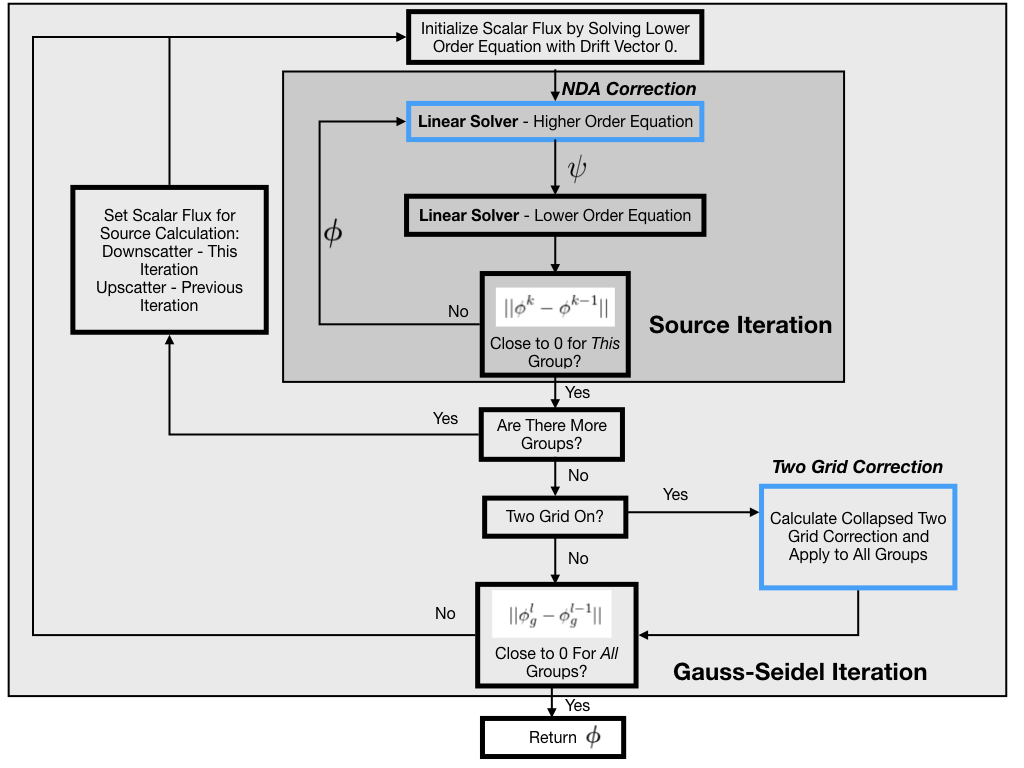
\includegraphics[width=\textwidth]{fig/TGNDAchart.png}
    \caption{Full Iterative TG-NDA Scheme}
    \label{fig:tgnda-graph}
\end{figure}